% Chapter 11

\chapter{Rendimiento} % Chapter title

\label{ch:rendimiento} % For referencing the chapter elsewhere, use \autoref{ch:name} 

Como parte de la metodología del presente proyecto se discutirán herramientas que permitirán realizar la medición de la eficiencia, en relación a la transferencia de información entre los clientes y un servidor. Esta medición se realizará en un ambiente definido en las siguientes secciones y además se creará una comparación entre el protocolo HTTP y un prototipo del protocolo CWC. 

Por otro lado como parte del análisis de costos se establecerá los requerimientos mínimos necesarios, para poder desarrollar los ambientes de pruebas. Ésta configuración de hardware conformará los parámetros para el cálculo de costo. 

%----------------------------------------------------------------------------------------

\section{Herrramientas}

%------------------------------------------------

\subsection{httperf}

Httperf es una herramienta para medir el rendimiento de aplicaciones web. Provee una manera flexibe de generar múltiples cargas de trabajo utilizando HTTP y con ellas poder medir el rendimiento Web. Puede observarse el funcionamiento de esta herramienta en la figura \ref{httperf}.

\begin{figure}[h]
  \centering
    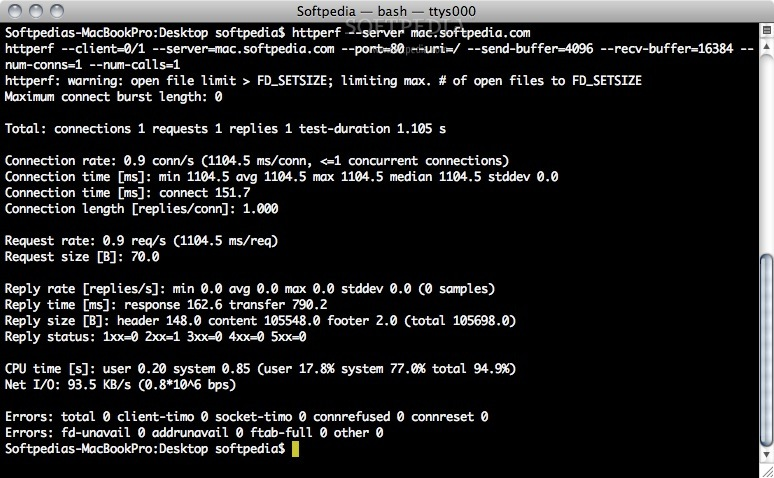
\includegraphics[scale=0.4]{gfx/httperf}
  \caption{Funcionamiento de httperf}
  \label{httperf}
\end{figure}

\subsection{OpenWebLoad}
OpenWebLoad es otra herramienta muy sencilla pero poderosa, es completamente en consola y permite hacer peticiones de archivos y entre la información que arroja esta número de ejecuciones, tiempo de respuesta de cada ejecución y tiempo de ejecución promedio. Puede observarse el funcionamiento de esta herramienta en la figura \ref{OpenWebLoad}.

\begin{figure}[h]
  \centering
    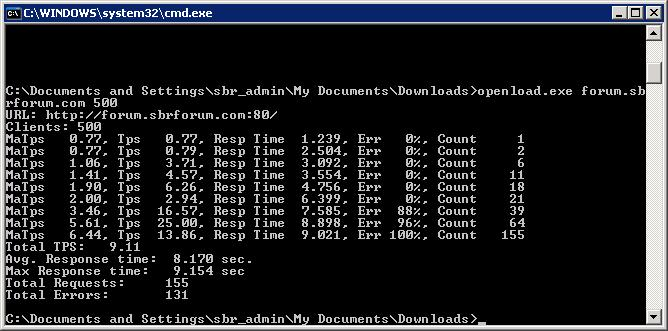
\includegraphics[scale=0.6]{gfx/OpenWebLoad}
  \caption{Funcionamiento de OpenWebLoad}
  \label{OpenWebLoad}
\end{figure}

\subsection{Time}
\label{subsec:time}
El comando time puede servir para obtener el tiempo que tarda una aplicación en completarse. En este caso se puede combinar con cualquier otra aplicación, por ejemplo con el prototipo del CWC. Puede observarse el funcionamiento de esta herramienta en la figura \ref{time}.

\begin{figure}[h]
  \centering
    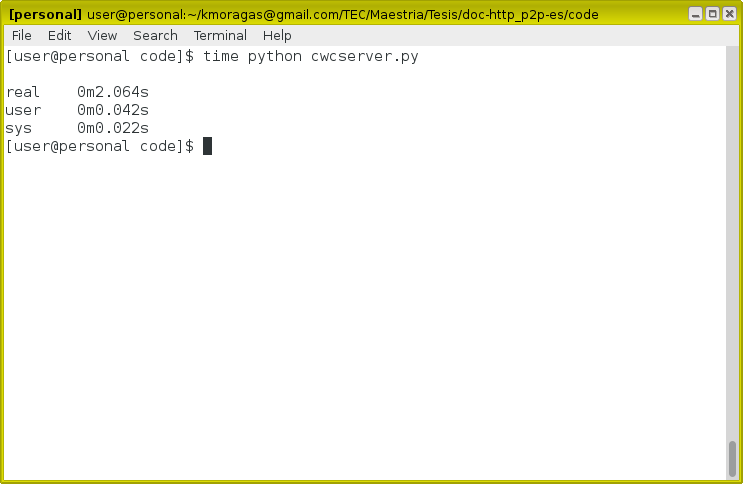
\includegraphics[scale=0.6]{gfx/time}
  \caption{Funcionamiento de time}
  \label{time}
\end{figure}

%------------------------------------------------

\subsection{JMeter}

JMeter forma del proyecto TomCat y es una herramienta muy utilizada para realizar pruebas de carga en un sitio web, mediante esta herramienta se puede describir prácticamente todo el comportamiento de un usuario dentro de un sitio web, desde cuando se autentica hasta cuando se llenan campos de texto en un formulario. Puede observarse el funcionamiento de esta herramienta en la figura \ref{jmeter}.

\begin{figure}[h]
  \centering
    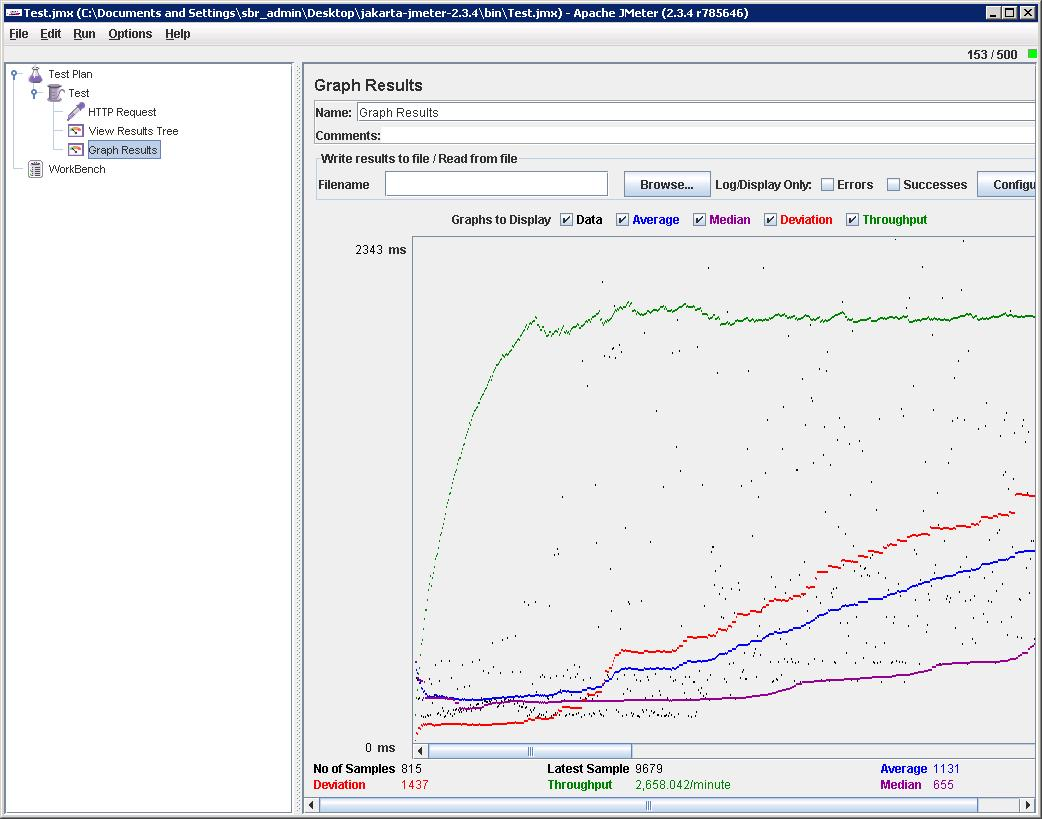
\includegraphics[scale=0.4]{gfx/jmeter}
  \caption{Resultados de Tiempo de Respuesta}
  \label{jmeter}
\end{figure}



%----------------------------------------------------------------------------------------

\section{Parámetros de las pruebas}
\label{sec:parametros_pruebas}

\subsection{Servidor Web y Servidor Caché}
\label{subsec:servidor_web}
El servidor web que utilizará será Apache, la configuración de éste deberá ser:

\begin{itemize}
\item GNU/Linux Debian Wheezy.
\item Apche2.2 con la instalación por defecto.
\item 4GB de RAM 
\item Dos núcleos
\item Al menos 100MB de espacio disponible.
\item Una interfaz de red.
\end{itemize}

Los valores de la configuración fueron tomados, basados en los recursos mínimos que se pueden adquirir a través de un sitio común de venta de dispositivos electrónicos. 

\subsection{Tipos de archivos de prueba}
\label{subsec:archivos}
En este caso se utilizarán archivos de diferente tipo y de diferente tamaño para realizar las pruebas, entre los tipos de archivos que se utilizarán son:

\begin{itemize}
\item Imágenes JPEG, PNG y GIF
\item Videos FLV, mpeg y AVI
\item Documentos ODT, DOC y XSLT
\item Instaladores EXE, BIN, MSI, DEB, RPM
\end{itemize}

Los tamaños de los archivos variarán, el máximo tamaño deberá ser de 600MB y el mínimo de de 1MB.

\subsection{Estrategia de las pruebas}
\label{subsec:estrategia_pruebas}
Como parte de la estrategia se limitará el ancho de banda a 200 KB/s en cada servidor. Además las pruebas que se deben ejecutar son:

\begin{itemize}
\item Con archivos pequeños, tamaños menores a los 100MB.
\item Archivos Grandes, tamaños superiores a 100MB.
\item Por tipo de archivo.
\item Todos los archivos.
\end{itemize}

\section{Escenarios}
\label{sec:escenarios}

\begin{description}
\item[Sin Web Caché] Este es el modelo tradicional de HTTP en el cual se tiene un sólo servidor web y múltiples clientes se conecta a él. En el caso de la prueba se configurará confirme a lo definido en la sección \ref{subsec:servidor_web}, además se configurará un límite de transferencia entre el servidor y el cliente definido en la sección de estretegia de pruebas ubicada en el apartado \ref{subsec:estrategia_pruebas}. Por otro lado, este servidor servirá los archivos definidos en la sección \ref{subsec:archivos}.

\item [Prototipo de CWC] Se medirá el comportamiento de la transferencia a través del prototipo de CWC. Los archivos a medir son igualmente los defindos en la sección  \ref{subsec:archivos}. Por otro lado la configuración de hardware por cada nodo será la misma que se presenta en la sección \ref{subsec:servidor_web}, pero en éste caso no será necesario configurar ningún servidor web en el sistema. También se limitará el ancho de banda entre los nodos y el cliente.
\end{description}
